\documentclass[uplatex, 12pt, dvipdfmx]{jsarticle}
\title{ことば}
\author{司馬 博文}
\date{\today}
\pagestyle{empty} \setcounter{secnumdepth}{4}
\input{/Users/hirofumi.shiba48/Desktop/数理科学/preamble.tex}
\usetikzlibrary{positioning,automata}
\begin{document}


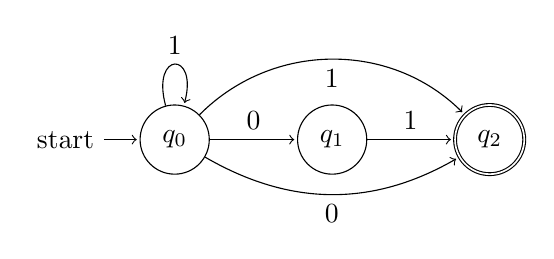
\begin{tikzpicture}[shorten >=1pt,node distance=2cm,on grid]
    \node[state,initial]   (q_0)                {$q_0$};
    \node[state]           (q_1) [right=of q_0] {$q_1$};
    \node[state,accepting] (q_2) [right=of q_1] {$q_2$};
    \path[->] (q_0) edge                node [above] {0} (q_1)
                    edge [loop above]   node         {1} ()
                    edge [bend left=45] node [below] {1} (q_2)
                    edge [bend right]   node [below] {0} (q_2)
              (q_1) edge                node [above] {1} (q_2);
\end{tikzpicture}

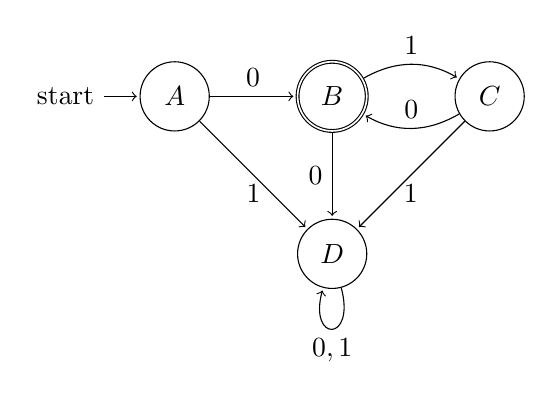
\begin{tikzpicture}[shorten >=1pt,node distance=2cm,on grid]
    \node[state,initial]   (A)                {$A$};
    \node[state,accepting] (B) [right=of A]   {$B$};
    \node[state]           (C) [right=of B]   {$C$};
    \node[state]           (D) [below=of B]    {$D$};
    \path[->] (A) edge                  node [above] {$0$} (B)
                  edge                  node [below] {$1$} (D)
              (B) edge [bend left]      node [above] {$1$} (C)
                  edge                  node [left] {$0$} (D)
              (C) edge [bend left]      node [above] {$0$} (B)
                  edge                  node [below] {$1$} (D)
              (D) edge [loop below]     node         {$0,1$} ();
\end{tikzpicture}

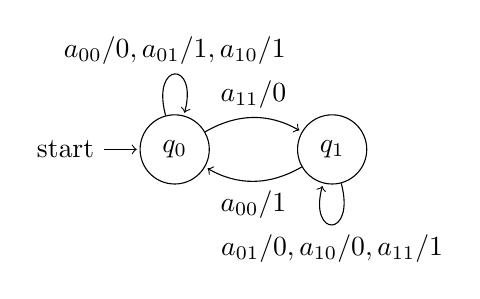
\begin{tikzpicture}[shorten >=1pt,node distance=2cm,on grid]
    \node[state,initial]   (q_0)        {$q_0$};
    \node[state]           (q_1) [right=of q_0]        {$q_1$};
    \path[->] (q_0) edge [bend left]    node [above] {$a_{11}/0$} (q_1)
                    edge [loop above]   node [above] {$a_{00}/0,a_{01}/1,a_{10}/1$} ()
              (q_1) edge [bend left]    node [below] {$a_{00}/1$} (q_0)
                    edge [loop below]   node [below] {$a_{01}/0,a_{10}/0,a_{11}/1$} ();
\end{tikzpicture}

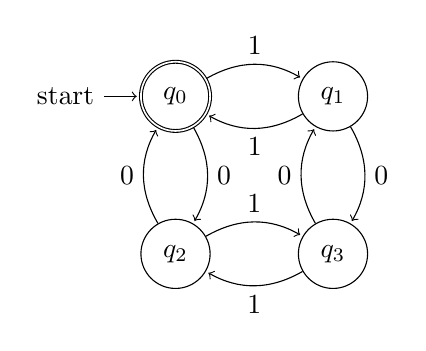
\begin{tikzpicture}[shorten >=1pt,node distance=2cm,on grid]
    \node[state,initial,accepting]   (q_0)        {$q_0$};
    \node[state]           (q_1) [right=of q_0] {$q_1$};
    \node[state]           (q_2) [below=of q_0] {$q_2$};
    \node[state]           (q_3) [right=of q_2] {$q_3$};
    \path[->] (q_0) edge [bend left]    node [above] {$1$} (q_1)
                    edge [bend left]    node [right] {$0$} (q_2)
              (q_1) edge [bend left]    node [below] {$1$} (q_0)
                    edge [bend left]    node [right] {$0$} (q_3)
              (q_2) edge [bend left]    node [left]  {$0$} (q_0)
                    edge [bend left]    node [above] {$1$} (q_3)
              (q_3) edge [bend left]    node [left]  {$0$} (q_1)
                    edge [bend left]    node [below] {$1$} (q_2);
\end{tikzpicture}

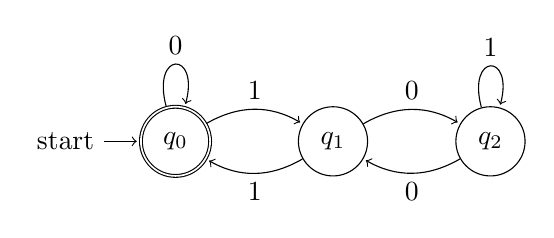
\begin{tikzpicture}[shorten >=1pt,node distance=2cm,on grid]
    \node[state,initial,accepting]   (q_0)        {$q_0$};
    \node[state]           (q_1) [right=of q_0] {$q_1$};
    \node[state]           (q_2) [right=of q_1] {$q_2$};
    \path[->] (q_0) edge [bend left]    node [above] {$1$} (q_1)
                    edge [loop above]    node [above] {$0$} ()
              (q_1) edge [bend left]    node [below] {$1$} (q_0)
                    edge [bend left]    node [above] {$0$} (q_2)
              (q_2) edge [bend left]    node [below]  {$0$} (q_1)
                    edge [loop above]    node [above] {$1$} ();
\end{tikzpicture}

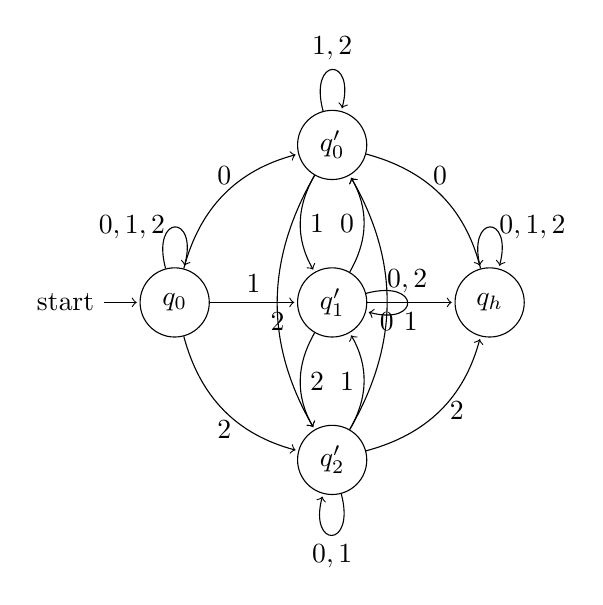
\begin{tikzpicture}[shorten >=1pt,node distance=2cm,on grid]
    \node[state,initial]   (q_0)        {$q_0$};
    \node[state]           (q'_1) [right=of q_0] {$q'_1$};
    \node[state]           (q'_2) [below=of q'_1] {$q'_2$};
    \node[state]           (q'_0) [above=of q'_1] {$q'_0$};
    \node[state]           (q_h)  [right=of q'_1] {$q_h$};
    \path[->] (q_0) edge [bend left]    node [above] {$0$} (q'_0)
                    edge                node [above] {$1$} (q'_1)
                    edge [bend right]    node [below] {$2$} (q'_2)
                    edge [loop above]    node [left] {$0,1,2$} ()
              (q'_0) edge [bend left]    node [above] {$0$} (q_h)
                    edge [bend right]    node [below] {$2$} (q'_2)
                    edge [bend right]    node [right] {$1$} (q'_1)
                    edge [loop above]    node [above] {$1,2$} ()
              (q'_1) edge               node  [below] {$1$} (q_h)
                    edge [bend right]    node [left] {$0$} (q'_0)
                    edge [bend right]    node [right] {$2$} (q'_2)
                    edge [loop right]    node [above] {$0,2$} ()
              (q'_2) edge [bend right]    node [below]  {$0$} (q'_0)
                    edge [bend right]    node [left] {$1$} (q'_1)
                    edge [bend right]    node [right] {$2$} (q_h)
                    edge [loop below]    node [below] {$0,1$} ()
              (q_h) edge [loop above]    node [right] {$0,1,2$} ();
\end{tikzpicture}

\[\begin{array}{c|cccc}
    &\multicolumn{4}{c}{入力}\\
    \cline{2-5}状態&0&1&2&\epsilon\\\hline
    q_0&\{q_0\}&\emptyset&\emptyset&\{q_1\}\\
    q_1&\emptyset&\{q_1\}&\emptyset&\{q_2\}\\
    q_2&\emptyset&\emptyset&\{q_2\}&\emptyset\\\hline
\end{array}\]

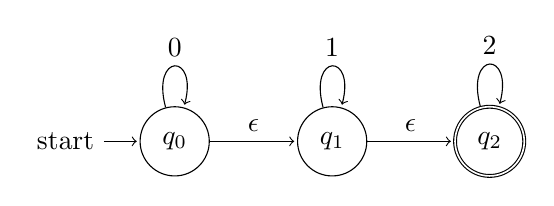
\begin{tikzpicture}[shorten >=1pt,node distance=2cm,on grid]
    \node[state,initial]   (q_0)        {$q_0$};
    \node[state]           (q_1) [right=of q_0] {$q_1$};
    \node[state,accepting]           (q_2) [right=of q_1] {$q_2$};
    \path[->] (q_0) edge                  node [above] {$\epsilon$} (q_1)
                    edge [loop above]    node [above] {$0$} ()
              (q_1) edge [loop above]    node [above] {$1$} ()
                    edge                 node [above] {$\epsilon$} (q_2)
              (q_2) edge [loop above]    node [above] {$2$} ();
\end{tikzpicture}

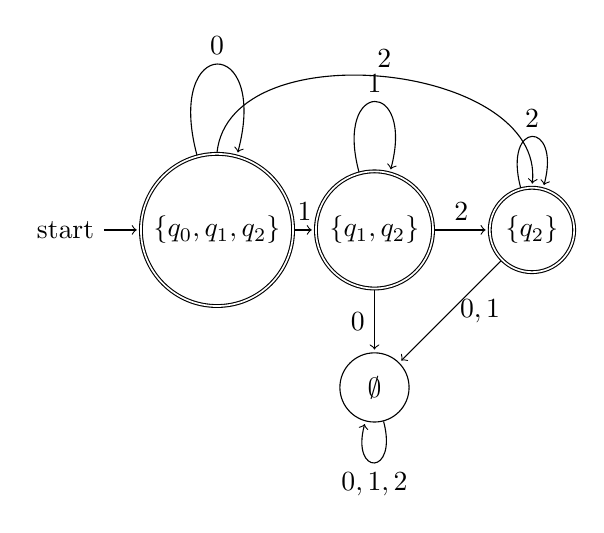
\begin{tikzpicture}[shorten >=1pt,node distance=2cm,on grid]
    \node[state,initial,accepting]   (q_0)        {$\{q_0,q_1,q_2\}$};
    \node[state,accepting]           (q_1) [right=of q_0] {$\{q_1,q_2\}$};
    \node[state,accepting]           (q_2) [right=of q_1] {$\{q_2\}$};
    \node[state]           (empty) [below=of q_1] {$\emptyset$};
    \path[->] (q_0) edge                  node [above] {$1$} (q_1)
                    edge [loop above]    node [above] {$0$} ()
                    edge [bend left=90]     node [above] {$2$} (q_2)
              (q_1) edge [loop above]    node [above] {$1$} ()
                    edge                 node [above] {$2$} (q_2)
                    edge                 node [left]  {$0$} (empty)
              (q_2) edge [loop above]    node [above] {$2$} ()
                    edge                 node [right] {$0,1$} (empty)
              (empty) edge [loop below]  node [below] {$0,1,2$} ();
\end{tikzpicture}

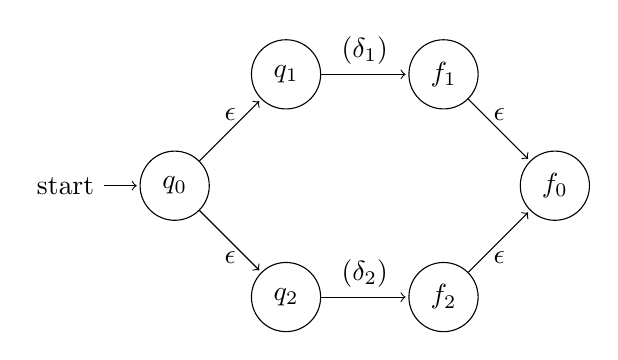
\begin{tikzpicture}[shorten >=1pt,node distance=2cm,on grid]
    \node[state,initial]   (q_0)        {$q_0$};
    \node[state]           (q_1) [above right=of q_0] {$q_1$};
    \node[state]           (q_2) [below right=of q_0] {$q_2$};
    \node[state]           (f_1) [right=of q_1] {$f_1$};
    \node[state]           (f_2) [right=of q_2] {$f_2$};
    \node[state]           (f_0) [below right=of f_1] {$f_0$};
    \path[->] (q_0) edge                  node [above] {$\epsilon$} (q_1)
                    edge                  node [below] {$\epsilon$} (q_2)
              (q_1) edge                  node [above] {$(\delta_1)$} (f_1)
              (q_2) edge                  node [above] {$(\delta_2)$} (f_2)
              (f_1) edge                  node [above] {$\epsilon$} (f_0)
              (f_2) edge                  node [below] {$\epsilon$} (f_0);
\end{tikzpicture}

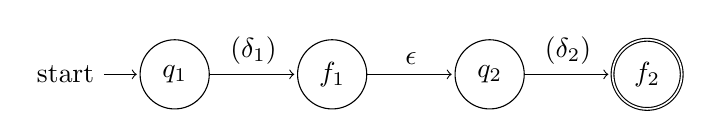
\begin{tikzpicture}[shorten >=1pt,node distance=2cm,on grid]
    \node[state,initial]   (q_1)        {$q_1$};
    \node[state]           (f_1) [right=of q_1] {$f_1$};
    \node[state]           (q_2) [right=of f_1] {$q_2$};
    \node[state,accepting]           (f_2) [right=of q_2] {$f_2$};
    \path[->] (q_1) edge                  node [above] {$(\delta_1)$} (f_1)
              (f_1)  edge                 node [above] {$\epsilon$} (q_2)
              (q_2) edge                  node [above] {$(\delta_2)$} (f_2);
\end{tikzpicture}

\begin{tikzpicture}[shorten >=1pt,node distance=2cm,on grid]
    \node[state,initial]   (q_0)        {$q_0$};
    \node[state]           (q_1) [right=of q_0] {$q_1$};
    \node[state]           (f_1) [right=of q_1] {$f_1$};
    \node[state,accepting]           (f_0) [right=of f_1] {$f_0$};
    \path[->] (q_0) edge                  node [above] {$\epsilon$} (q_1)
                    edge  [bend right=45] node [below] {$\epsilon$} (f_0)
              (q_1)  edge                 node [above] {$(\delta_1)$} (f_1)
              (f_1) edge                  node [above] {$\epsilon$} (f_2)
                    edge [bend right=45]                 node [above] {$\epsilon$} (q_1);
\end{tikzpicture}



\end{document}